\documentclass[titlepage]{scrartcl}
\usepackage{enumitem}
\usepackage[british]{babel}
\usepackage[style=apa, backend=biber]{biblatex}
\DeclareLanguageMapping{british}{british-apa}
\usepackage{url}
\usepackage{float}
\usepackage[labelformat=empty]{caption}
\restylefloat{table}
\usepackage{perpage}
\MakePerPage{footnote}
\usepackage{abstract}
\usepackage{graphicx}
% Create hyperlinks in bibliography
\usepackage{hyperref}
\usepackage{amsmath}

\usepackage[T1]{fontenc}
\usepackage[utf8]{inputenc}
\usepackage{blindtext}
\setkomafont{disposition}{\normalfont\bfseries}

\graphicspath{
    {./resources/},
}
\addbibresource{~/Documents/library.bib}

\newsavebox{\abstractbox}
\renewenvironment{abstract}
  {\begin{lrbox}{0}\begin{minipage}{\textwidth}
   \begin{center}\normalfont\sectfont\abstractname\end{center}\quotation}
  {\endquotation\end{minipage}\end{lrbox}%
   \global\setbox\abstractbox=\box0 }

\usepackage{etoolbox}
\makeatletter
\expandafter\patchcmd\csname\string\maketitle\endcsname
  {\vskip\z@\@plus3fill}
  {\vskip\z@\@plus2fill\box\abstractbox\vskip\z@\@plus1fill}
  {}{}
\makeatother

\DeclareCiteCommand{\citeyearpar}
    {}
    {\mkbibparens{\bibhyperref{\printdate}}}
    {\multicitedelim}
    {}

\begin{document}
    \title{ECS742\\Interactive Digital Media Techniques\\Mini-Assignment 1: Arduino}
    \subtitle{\LARGE{Technical Report}}
    \author{Sam Perry\\160842984}
    \date{}
    \maketitle

    \section{Connecting and Reading the FSR}
    Initially, a circuit was created to demonstrate the reading of values from
    the FSR (Force Sensitive Resistor).  A 5V supply was used to pass a current
    through the resistor, which was measured via analog input 0.  A 10kohm
    pulldown resistor was conntected to ground between the FSR and the input.
    This was necessary to avoid a direct connection between the 5V supply and
    ground at points when the FSR provides little to no resistance. This also
    creates a consistantly low value to input when resistance from the FSR
    is high, avoiding unpredicatbale floating readings caused by a disconected
    input.\\

    Code was written to print values to the serial port. A Python script was
    used to record these values as shown:

    
    \begin{figure}[H]
        \caption{Value measured over time. A sharp increase in preassure followed by a gradual release is displayed.}
        \makebox[\textwidth]{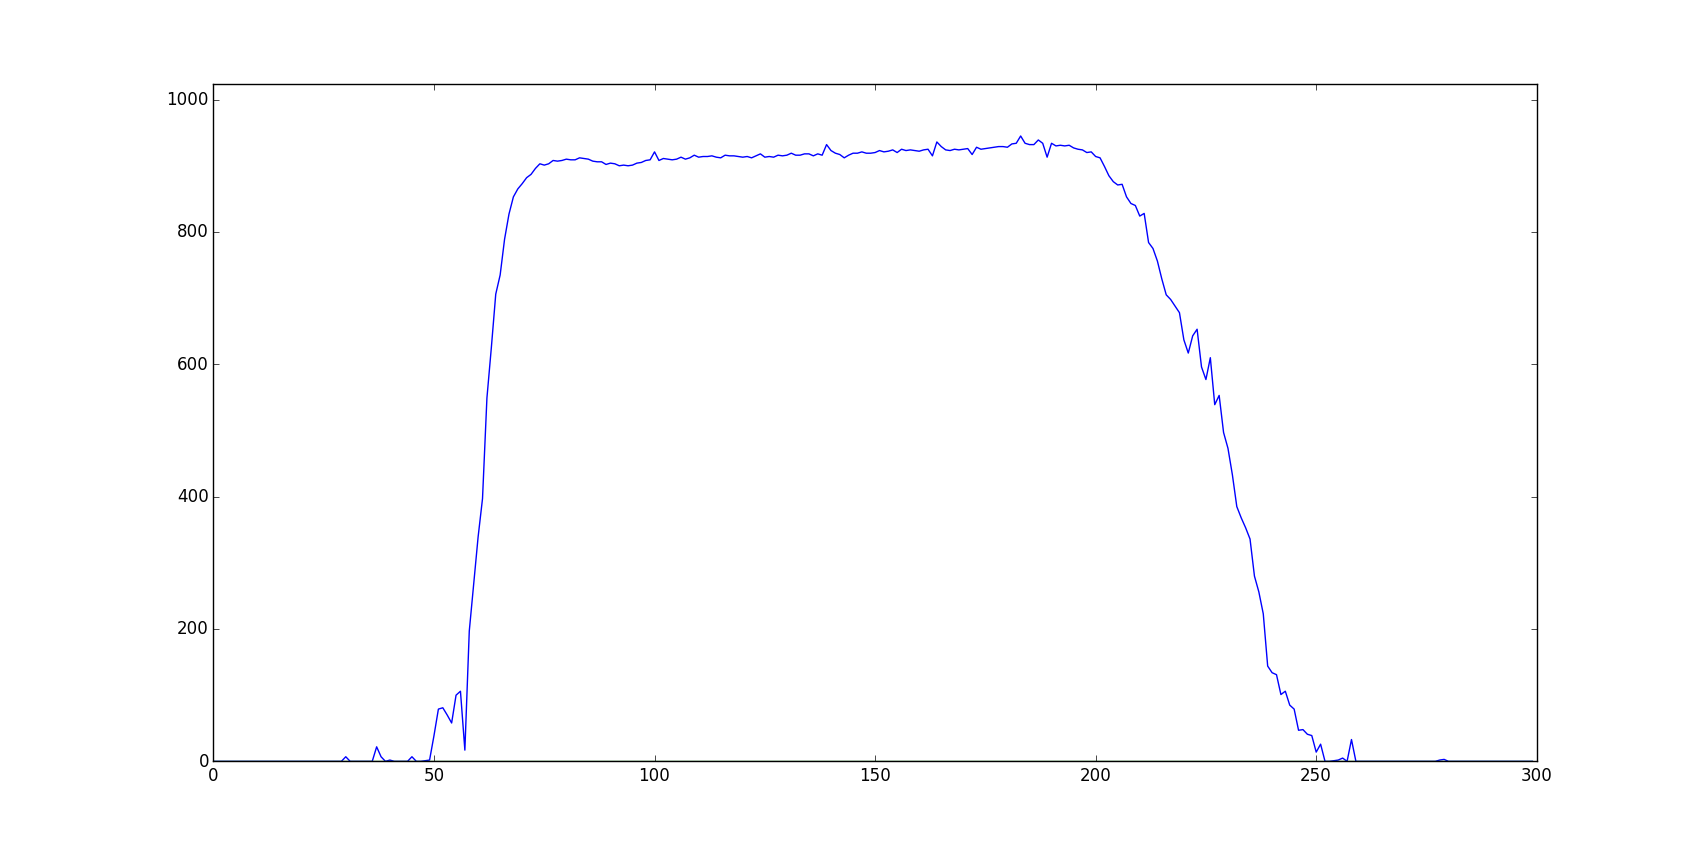
\includegraphics[width=0.75\textwidth]{FSR_Linearity}}
    \end{figure}

    From these readings it can be seen that there is a non-linear relationship
    between applied preassure and measurement. As the voltage measured is
    proportional to the inverse of the FSR resistance \parencite{ada2016},
    voltage increases at what appears to be an exponentially decreasing rate as
    resistance increase at the same rate.

    \section{Using the FSR Values To Create a Tone}
    \section{Using the Buttons to Make a Simple Keyboard}
    \section{Adding Vibrato Using the FSR}

    \printbibliography
\end{document}
